\chapter{Proper Time, Time Dilation, and Length Contraction}

We shall often choose units in which the speed of light is $c=1$. In those
units a year of time and a light-year of distance may be compared directly,
and the formulas are much easier to read. Whenever $c$ matters physically,
we shall put it back. Dimensional analysis is enough to locate it.

\section{The Galilean Spacetime Grid}

Begin with the pre-Einstein relation between a frame at rest and a train moving
at velocity $v$ along the $x$-axis:
\begin{align}
x' &= x-vt, & t'&=t.
\label{eq:l4-galilean}
\end{align}
The second equation contains Newton's assumption of universal time. Every
observer uses the same simultaneity slices, even though the spatial origins
move relative to one another.

Suppose the unprimed observer stands beside the track and the primed observer
rides the train. The train's origin has $x'=0$, so its worldline in the
unprimed coordinates is
\begin{equation}
x=vt.
\end{equation}
That sloping line is the $t'$-axis. By contrast, $t'=t$ says that all lines
of constant $t'$ are the same horizontal lines as those of constant $t$.

\begin{figure}[H]
\centering

\includegraphics[width=0.72\textwidth]{lecture_04_figure_02.png}
\caption{The Galilean transformation and the initial $t$-$x$ grid. The
moving origin will trace $x=vt$, while the two frames retain common
constant-time lines.}
\lectureframe{00:03:06}
\end{figure}

Solving Eq.~\eqref{eq:l4-galilean} for the unprimed coordinates gives
\begin{align}
x&=x'+vt'=x'+vt, & t&=t'.
\end{align}
The inverse has the same form with $v$ replaced by $-v$. If the train moves
forward relative to the station, the station moves backward relative to the
train. This reciprocity survives in special relativity, but universal time
does not.

\section{The Lorentz Correction}

Galilean transformations cannot make the speed of light the same in every
inertial frame. The corrected relations are, first in $c=1$ units,
\begin{align}
x'&=\frac{x-vt}{\sqrt{1-v^2}}, &
t'&=\frac{t-vx}{\sqrt{1-v^2}}.
\label{eq:l4-lorentz-natural}
\end{align}
Restoring ordinary units gives
\begin{align}
x'&=\frac{x-vt}{\sqrt{1-v^2/c^2}}, &
t'&=\frac{t-vx/c^2}{\sqrt{1-v^2/c^2}}.
\label{eq:l4-lorentz-c}
\end{align}

\begin{figure}[H]
\centering

\includegraphics[width=0.74\textwidth]{lecture_04_figure_05.png}
\caption{The Lorentz transformation with the factors of $c$ restored.}
\lectureframe{00:09:10}
\end{figure}

For $v\ll c$, both $v^2/c^2$ and $vx/c^2$ are tiny in the circumstances
where Newtonian mechanics is used. Equation~\eqref{eq:l4-lorentz-c} then
reduces to the Galilean result. Relativity does not discard Newtonian
kinematics; it identifies its range of validity.

At $v=c$, the denominator vanishes. An inertial frame cannot move at the
speed of light relative to another inertial frame. Well below that limit the
corrections are small, but near it the mixing of $x$ and $t$ becomes
unavoidable.

Motion was chosen along $x$, so the transverse coordinates do not change:
\begin{equation}
y'=y,\qquad z'=z.
\end{equation}
One way to see why is to place identical transverse meter sticks on the train
and platform. An observer moving halfway between the two frames sees the rods
approach with equal and opposite speeds. The setup has no feature that could
make one transverse rod shorter than the other.

\section{Lorentz Transformations Along the Light Cone}

There is a geometric way to read Eq.~\eqref{eq:l4-lorentz-natural}. Add its
two equations:
\begin{align}
t'+x'
&=\frac{(t-vx)+(x-vt)}{\sqrt{1-v^2}}\\
&=(t+x)\frac{1-v}{\sqrt{1-v^2}}\\
&=(t+x)\sqrt{\frac{1-v}{1+v}}.
\label{eq:l4-null-plus}
\end{align}
Subtract them in the complementary order:
\begin{align}
t'-x'
&=\frac{(t-vx)-(x-vt)}{\sqrt{1-v^2}}\\
&=(t-x)\frac{1+v}{\sqrt{1-v^2}}\\
&=(t-x)\sqrt{\frac{1+v}{1-v}}.
\label{eq:l4-null-minus}
\end{align}

\begin{figure}[H]
\centering

\includegraphics[width=0.75\textwidth]{lecture_04_figure_06.png}
\caption{The Lorentz transformation rewritten in the null combinations
$t+x$ and $t-x$. Their scale factors are reciprocal.}
\lectureframe{00:18:45}
\end{figure}

The combinations $t+x$ and $t-x$ are coordinates along the two
$45^\circ$ lightlike directions. A boost squeezes one of these directions
and stretches the other by the inverse factor. It does not rotate either one
away from $45^\circ$. Thus light rays remain light rays, which is the
spacetime picture of the invariant speed of light.

\begin{classroomqa}
\audiencequestion{The halfway observer sees a symmetric experiment, but how
does that establish the result for the train and platform observers?
\lecturetimestamp{00:20:48}}
\lecturerresponse{One additional fact is being used: a coincidence of events
is invariant. If the ends of the rods meet, that meeting is one spacetime
event. Every inertial observer may assign different coordinates to it, but
none may split one coincidence into two different locations. Flashes emitted
where the corresponding endpoints meet make those events operationally
detectable. The symmetry of the halfway frame and the invariance of the two
endpoint coincidences establish that the transverse lengths agree.}
\end{classroomqa}

\begin{classroomqa}
\audiencequestion{Must the bicyclist who represents the halfway frame be
located physically at the midpoint of the rods?\lecturetimestamp{00:22:25}}
\lecturerresponse{No. A reference frame is a whole network of observers and
clocks, not one eye at one place. The bicyclist may receive the endpoint
flashes later and infer where they originated. What matters is the spacetime
location of each emission event, not where the light is eventually received.}
\end{classroomqa}

The composition of successive velocities is another consequence of the same
transformation, but it is deliberately left for the next lecture. The present
task is to identify the invariant quantity that a moving clock measures.

\section{The Invariant Interval}

For a rotation of ordinary Cartesian axes, the quantity $x^2+y^2$ is
unchanged. Lorentz transformations preserve a different quadratic form. From
Eq.~\eqref{eq:l4-lorentz-natural},
\begin{align}
t'^2-x'^2
&=\frac{(t-vx)^2-(x-vt)^2}{1-v^2}\\
&=\frac{t^2-2vtx+v^2x^2-x^2+2vtx-v^2t^2}{1-v^2}\\
&=t^2-x^2.
\label{eq:l4-interval}
\end{align}
The mixed terms cancel, and the remaining numerator contains a common factor
of $1-v^2$.

\begin{figure}[H]
\centering

\includegraphics[width=0.76\textwidth]{lecture_04_figure_07.png}
\caption{The board derivation of $t'^2-x'^2=t^2-x^2$.}
\lectureframe{00:33:15}
\end{figure}

With three spatial dimensions the invariant is
\begin{equation}
t'^2-x'^2-y'^2-z'^2=t^2-x^2-y^2-z^2
\end{equation}
in $c=1$ units. More generally, for two events we use coordinate
differences:
\begin{equation}
\Delta s^2
=c^2\Delta t^2-\Delta x^2-\Delta y^2-\Delta z^2.
\label{eq:l4-spacetime-interval}
\end{equation}
Every inertial observer agrees on this number even though they disagree on
its separate time and space terms.

\section{Proper Time and Moving Clocks}

Imagine a lattice of stationary observers whose clocks have been synchronized
by exchanging light signals. Their readings define the coordinate time $t$.
Now carry one wristwatch through that lattice. Its own reading follows the
watch along its worldline; that reading is proper time.

For two timelike-separated events, define
\begin{equation}
c^2\Delta\tau^2
=c^2\Delta t^2-\Delta x^2-\Delta y^2-\Delta z^2.
\label{eq:l4-proper-time}
\end{equation}
In one spatial dimension with $c=1$, this is simply
\begin{equation}
\Delta\tau=\sqrt{\Delta t^2-\Delta x^2}.
\end{equation}
The square root parallels the formula for an ordinary distance, but the minus
sign changes the geometry.

There are three cases:
\begin{align}
\Delta t^2-\Delta x^2 &>0 &&\text{timelike},\\
\Delta t^2-\Delta x^2 &=0 &&\text{lightlike},\\
\Delta t^2-\Delta x^2 &<0 &&\text{spacelike}.
\end{align}
Inside the light cone the proper time is real. On the cone, where
$x=\pm t$, it is zero even though the events need not coincide. A light ray
can connect precisely such events. Outside the cone the separation is
spacelike; it is better to describe it by the real proper distance
$\sqrt{\Delta x^2-\Delta t^2}$ than by an imaginary clock time.

\begin{figure}[H]
\centering

\includegraphics[width=0.73\textwidth]{lecture_04_figure_08.png}

\vspace{0.8em}

\begin{tikzpicture}[x=1.0cm,y=1.0cm]
\draw[->] (-3.3,0) -- (3.3,0) node[right] {$x$};
\draw[->] (0,-0.4) -- (0,4.0) node[above] {$t$};
\draw[thick] (0,0) -- (3.0,3.0) node[above right] {$x=t$};
\draw[thick] (0,0) -- (-3.0,3.0) node[above left] {$x=-t$};
\node at (0,2.0) {timelike};
\node at (2.25,1.05) {spacelike};
\node at (-2.25,1.05) {spacelike};
\end{tikzpicture}
\caption{The board light cone and a clean classification of timelike,
lightlike, and spacelike separation.}
\lectureframe{00:38:40}
\end{figure}

Why does Eq.~\eqref{eq:l4-proper-time} equal a clock reading? For a clock at
rest, $\Delta x=0$, so $\Delta\tau=\Delta t$. For a uniformly moving
clock, choose the primed frame in which that clock is at rest. There
$\Delta x'=0$, and invariance gives
\begin{equation}
\Delta\tau
=\sqrt{\Delta t'^2-\Delta x'^2}
=\Delta t'.
\end{equation}
Moving clocks therefore tick off proper time.

\begin{classroomqa}
\audiencequestion{Are ``the interval between the events'' and ``the reading
of the clock'' being used as two names for the same thing?
\lecturetimestamp{00:44:49}}
\lecturerresponse{They coincide when an ideal clock travels inertially from
one event to the other. The invariant interval is a geometric quantity; the
difference between the endpoint readings of the comoving clock is its physical
measurement. A stationary coordinate clock generally records a different
coordinate-time interval.}
\end{classroomqa}

\section{Time Dilation and Simultaneity}

Consider the origin of the moving frame. Its worldline obeys
\begin{equation}
x'=0,\qquad x=vt.
\end{equation}
The same sloping line is both the path of the moving clock and the $t'$-axis.

\begin{figure}[H]
\centering

\includegraphics[width=0.72\textwidth]{lecture_04_figure_03.png}
\caption{The moving origin: $x=vt$, $x'=0$, and the $t'$-axis are three
descriptions of the same worldline.}
\lectureframe{00:48:18}
\end{figure}

Apply the invariant interval between the common origin and a later point on
that worldline:
\begin{align}
t'^2-x'^2&=t^2-x^2,\\
t'^2&=t^2-v^2t^2,\\
t'&=t\sqrt{1-v^2}.
\label{eq:l4-time-dilation-natural}
\end{align}
With $c$ restored,
\begin{equation}
\Delta\tau=\Delta t\sqrt{1-\frac{v^2}{c^2}}
=\frac{\Delta t}{\gamma},
\qquad
\gamma=\frac{1}{\sqrt{1-v^2/c^2}}.
\label{eq:l4-time-dilation}
\end{equation}

\begin{figure}[H]
\centering

\includegraphics[width=0.73\textwidth]{lecture_04_figure_09.png}
\caption{The time-dilation result on the board: the moving clock accumulates
$t'=t\sqrt{1-v^2}$ in units with $c=1$.}
\lectureframe{00:50:45}
\end{figure}

The stationary observer says that the moving clock runs slow. Reciprocity
requires the moving observer to say the same about stationary clocks. There
is no contradiction because the two descriptions compare different pairs of
distant events.

Indeed, a constant value of $t'$ in
Eq.~\eqref{eq:l4-lorentz-natural} satisfies
\begin{equation}
t-vx=\text{constant}.
\label{eq:l4-simultaneity}
\end{equation}
The moving observer's simultaneity lines are tilted relative to the horizontal
lines $t=\text{constant}$. Each observer calls a different collection of
distant clock readings simultaneous. Once that difference is kept visible,
the reciprocal slowing of clocks is consistent.

\begin{figure}[H]
\centering
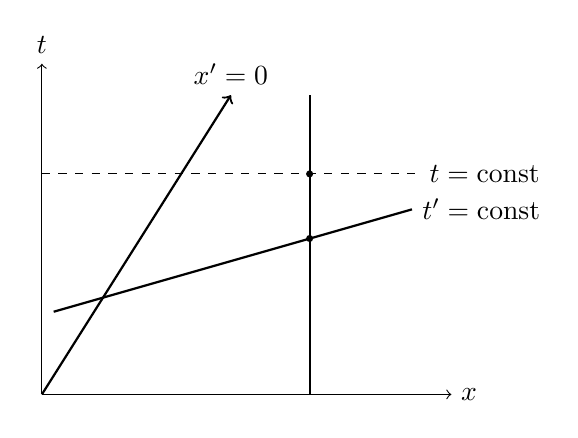
\begin{tikzpicture}[x=1cm,y=1cm]
\draw[->] (0,0) -- (0,4.2) node[above] {$t$};
\draw[->] (0,0) -- (5.2,0) node[right] {$x$};
\draw[thick,->] (0,0) -- (2.4,3.8) node[above] {$x'=0$};
\draw[dashed] (0,2.8) -- (4.8,2.8)
  node[right] {$t=\mathrm{const}$};
\draw[thick] (0.15,1.05) -- (4.7,2.35)
  node[right] {$t'=\mathrm{const}$};
\draw[thick] (3.4,0) -- (3.4,3.8);
\fill (3.4,2.8) circle (0.045);
\fill (3.4,1.98) circle (0.045);
\end{tikzpicture}
\caption{Reciprocal time dilation compares clock readings on different
simultaneity slices.}
\end{figure}

\section{The Twin Paths}

Two twins begin at the same event. One remains at $x=0$. The other travels
outward at speed $v$, reverses direction, and returns at the same speed.
When they reunite they compare every physical process that can serve as a
clock: watches, heartbeats, metabolism, or aging itself.

Let each half of the trip take coordinate time $T$ in the home frame. The
home twin's proper time is
\begin{equation}
\tau_{\mathrm{home}}=2T.
\end{equation}
The turn-around event has coordinates $(vT,T)$. The first traveling leg
therefore contributes
\begin{align}
\tau_{\mathrm{leg}}
&=\sqrt{T^2-v^2T^2}
=T\sqrt{1-v^2}.
\end{align}
The return leg contributes the same amount, hence
\begin{equation}
\tau_{\mathrm{travel}}=2T\sqrt{1-v^2}<2T.
\label{eq:l4-twin}
\end{equation}

\begin{figure}[H]
\centering

\includegraphics[width=0.73\textwidth]{lecture_04_figure_10.png}

\vspace{0.8em}

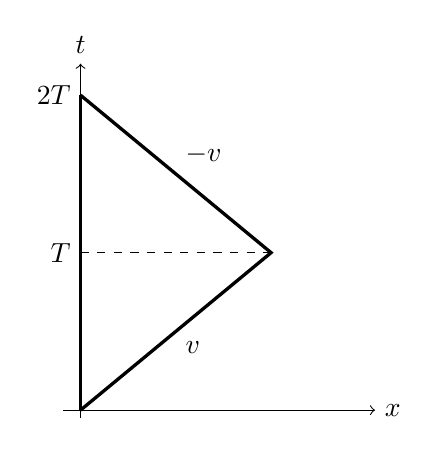
\begin{tikzpicture}[x=1.1cm,y=1cm]
\draw[->] (-0.2,0) -- (3.4,0) node[right] {$x$};
\draw[->] (0,-0.1) -- (0,4.4) node[above] {$t$};
\draw[very thick] (0,0) -- (0,4);
\draw[very thick] (0,0) -- (2.2,2) -- (0,4);
\draw[dashed] (0,2) -- (2.2,2);
\node[left] at (0,2) {$T$};
\node[left] at (0,4) {$2T$};
\node[below right] at (1.1,1.0) {$v$};
\node[above right] at (1.1,3.0) {$-v$};
\end{tikzpicture}
\caption{The home worldline and the two traveling legs. Their proper times
are different because they are different paths through spacetime.}
\lectureframe{00:59:35}
\end{figure}

There is no contradiction in the unequal ages. The traveling path contains a
turn and is not related to the straight home path by a single inertial-frame
symmetry. In ordinary Euclidean geometry a straight route and a broken route
between two points also have different lengths. Minkowski geometry reverses
which path has the larger interval, but the comparison is still geometric.

\section{Acceleration and the Ideal Clock}

\begin{classroomqa}
\audiencequestion{At the turn-around the physics is different and the traveler
accelerates. Does that invalidate the clock calculation?
\lecturetimestamp{01:02:19}}
\lecturerresponse{The acceleration is real and helps identify the asymmetry;
it should not be argued away. The sharp corner is only an idealized drawing
and may be rounded into a finite turn. The further physical assumption is
that a sufficiently small, well-built clock is insensitive to modest
acceleration and continues to record proper time. A large or fragile clock
may deform or break, but that is a defect of the mechanism rather than of the
spacetime interval.}
\end{classroomqa}

This ideal-clock assumption is not derived from the Lorentz transformation
alone. It is tested through the behavior of actual clock mechanisms. An atom
is a much better approximation than a clock hundreds of miles across because
the compact mechanism is harder to distort under acceleration or gravity.
Invoking general relativity by name would not eliminate this physical issue;
one would still have to know how the chosen mechanism responds to its
environment.

\begin{classroomqa}
\audiencequestion{Can an accelerated trajectory be reduced to short intervals
on which the inertial analysis remains valid?\lecturetimestamp{01:09:08}}
\lecturerresponse{Yes. Divide the curve into short, nearly straight segments,
calculate the proper time on each segment, and add the results. This is the
spacetime analogue of finding the length of an ordinary curve from many small
line segments. In the continuum limit,
\[
\tau=\int \sqrt{1-\frac{v(t)^2}{c^2}}\,dt,
\]
for motion in flat spacetime described in an inertial coordinate system.}
\end{classroomqa}

\section{What the Twins See}

The final clock readings can be made operational by sending light pulses. Mark
one-second intervals of proper time on both worldlines and let each twin emit
a pulse at every mark. During the outward leg, pulses received from the other
twin are spread apart. During the return, they arrive bunched together. This
is the relativistic Doppler effect expressed directly on the spacetime
diagram.

\begin{figure}[H]
\centering

\includegraphics[width=0.73\textwidth]{lecture_04_figure_11.png}
\caption{Light signals exchanged between the home and traveling worldlines.
Sparse arrivals on the outward leg and compressed arrivals on the return leg
account for every emitted pulse.}
\lectureframe{01:12:55}
\end{figure}

No frames of the story disappear. Each observer eventually receives all the
pulses emitted by the other, but their reception rates depend on the relative
motion. The outbound redshift and inbound blueshift are not equal-duration
effects for the two paths, so counting all received pulses agrees with the
proper-time comparison.

\begin{classroomqa}
\audiencequestion{If the returning traveler receives blueshifted light, could
the traveler collect more energy than the source emitted?
\lecturetimestamp{01:13:50}}
\lecturerresponse{That question requires the relativistic definition and
frame dependence of energy, which have not yet been developed. It is
reasonable, but coordinates and pulse counts alone are not enough to settle
the energy bookkeeping, especially for an accelerated observer. The answer
should therefore be postponed rather than guessed.}
\end{classroomqa}

\section{A Closed Spatial Direction}

\begin{classroomqa}
\audiencequestion{Suppose one spatial direction is compact. Could a twin move
uniformly around it, return to the starting place, and avoid acceleration
altogether? What then distinguishes the twins?\lecturetimestamp{01:15:14}}
\lecturerresponse{The space should be imagined intrinsically as a cylinder,
not as a sheet bent inside a larger space; there need be no radial
acceleration. The returning observer nevertheless encounters the global fact
that the same places recur. That indicates an asymmetry, but a complete answer
requires a careful treatment of special relativity with the spatial
identification. The question is left open here rather than answered
improvisationally.}
\end{classroomqa}

\begin{figure}[H]
\centering

\includegraphics[width=0.72\textwidth]{lecture_04_figure_04.png}

\vspace{0.8em}

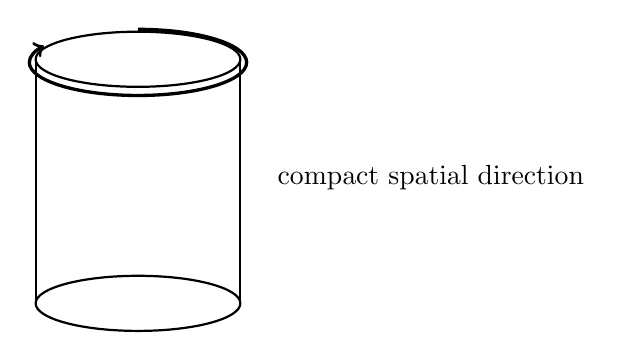
\begin{tikzpicture}[x=1cm,y=1cm]
\draw[thick] (0,0) ellipse (1.3 and 0.35);
\draw[thick] (-1.3,0) -- (-1.3,-3.1);
\draw[thick] (1.3,0) -- (1.3,-3.1);
\draw[thick] (0,-3.1) ellipse (1.3 and 0.35);
\draw[->,very thick] (0.0,0.38) arc (90:-210:1.38 and 0.42);
\node[right] at (1.65,-1.5) {compact spatial direction};
\end{tikzpicture}
\caption{The compact-space question as drawn on the board, with a clean
intrinsic cylinder. It is a question about global identification, not motion
around a cylinder embedded in an extra radial dimension.}
\lectureframe{01:17:56}
\end{figure}

\section{Length Is Measured on a Simultaneity Slice}

For a special-relativity problem, first draw the spacetime picture. Take a
meter stick at rest in the unprimed frame, with endpoints at $x=0$ and
$x=1$. As time passes, the two endpoints trace vertical worldlines. The
stick sweeps out a ribbon between them.

The moving observer must measure both endpoints at one value of the moving
time $t'$. From Eq.~\eqref{eq:l4-simultaneity}, the slice through the origin
with $t'=0$ satisfies
\begin{equation}
t=vx
\end{equation}
in $c=1$ units. It intersects the right endpoint $x=1$ at $t=v$.

\begin{figure}[H]
\centering

\includegraphics[width=0.73\textwidth]{lecture_04_figure_12.png}

\vspace{0.8em}

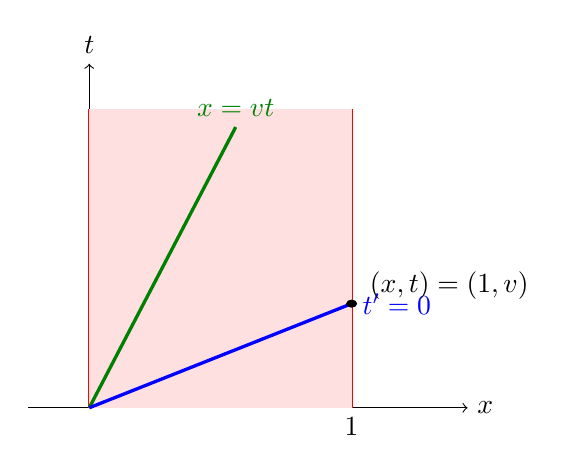
\begin{tikzpicture}[x=1.55cm,y=1.15cm]
\draw[->] (-0.5,0) -- (3.1,0) node[right] {$x$};
\draw[->] (0,0) -- (0,3.8) node[above] {$t$};
\draw[very thick,red] (0,0) -- (0,3.3);
\draw[very thick,red] (2.15,0) -- (2.15,3.3);
\fill[red!12] (0,0) rectangle (2.15,3.3);
\draw[very thick,green!50!black] (0,0) -- (1.2,3.1)
  node[above] {$x=vt$};
\draw[very thick,blue] (0,0) -- (2.15,1.15)
  node[right] {$t'=0$};
\fill (2.15,1.15) circle (0.045);
\node[right] at (2.22,1.35) {$(x,t)=(1,v)$};
\node[below] at (2.15,0) {$1$};
\end{tikzpicture}
\caption{A rod at rest sweeps out a spacetime ribbon. The moving observer's
length is the separation between its endpoints on one $t'=\mathrm{const}$
slice.}
\lectureframe{01:24:20}
\end{figure}

The selected endpoint separation is spacelike, so use the positive spatial
form of the invariant:
\begin{equation}
x'^2-t'^2=x^2-t^2.
\end{equation}
At the chosen endpoint, $t'=0$, $x=1$, and $t=v$. Hence
\begin{align}
x'^2&=1-v^2,\\
x'&=\sqrt{1-v^2}.
\end{align}
Thus a rest length $L$ is measured in the moving frame as
\begin{equation}
L'=L\sqrt{1-v^2/c^2}=\frac{L}{\gamma}.
\label{eq:l4-length-contraction}
\end{equation}

\begin{figure}[H]
\centering

\includegraphics[width=0.76\textwidth]{lecture_04_figure_13.png}
\caption{The completed length-contraction construction and the board result
$x'=\sqrt{1-v^2}$ for a unit rest length.}
\lectureframe{01:28:10}
\end{figure}

The reciprocal statement is also true: the platform observer assigns a
shorter length to the train's longitudinal meter stick. Once again the two
observers choose different simultaneous endpoint events, so reciprocity is
not contradictory.

\section{Questions at the End}

\begin{classroomqa}
\audiencequestion{Does anything besides light propagate at the speed of
light? In particular, what about gravity?\lecturetimestamp{01:29:29}}
\lecturerresponse{General relativity predicts gravitational waves that
propagate at $c$. At the time of this lecture, the evidence came indirectly
from systems such as binary pulsars; gravitational waves had not yet been
detected directly.\editorialnote{The experimental situation changed after
this 2006 lecture. LIGO directly detected GW150914 in 2015, and the joint
observation of GW170817 and its electromagnetic counterpart in 2017 showed
that the propagation speeds of gravity and light agree to within a few parts
in $10^{15}$. See \url{https://ligo.org/detections/gw150914/} and
\url{https://doi.org/10.1103/PhysRevLett.119.251302}.}}
\end{classroomqa}

\begin{classroomqa}
\audiencequestion{Can an astronaut cross a distance of many light-years in
less proper time than the distance expressed in light-years? Would that mean
moving faster than light?\lecturetimestamp{01:30:38}}
\lecturerresponse{The astronaut's proper time is
$\sqrt{\Delta t^2-\Delta x^2}$, which is smaller than the coordinate time
$\Delta t$. In the astronaut's inertial frame, the distance between the
stars is Lorentz-contracted. The stars move with speed $-v$, not faster than
light; there is simply less contracted distance to cross.}
\end{classroomqa}

If the astronaut begins at rest and accelerates, the description changes
between a succession of instantaneous inertial frames. The distance assigned
to the stars can change during that transition. One cannot apply one fixed
Lorentz transformation to the entire accelerated history, but the total
proper time still follows by adding the contributions along the worldline.
The same statement applies to a realistic twin who launches, turns, and
decelerates rather than being born at cruising speed.

\begin{classroomqa}
\audiencequestion{Are these puzzles caused by treating time as special? Must
we call it a fourth dimension?\lecturetimestamp{01:36:43}}
\lecturerresponse{It is not necessary to begin with the slogan that time is a
fourth dimension. The Lorentz transformation itself forces space and time to
mix, while the interval $t^2-x^2-y^2-z^2$ treats them as parts of one
geometry with a different sign for time and space. At low velocity the mixing
becomes negligible and familiar Newtonian intuition returns. At relativistic
velocity, however, space and time cannot be regarded as fundamentally
decoupled.}
\end{classroomqa}

Time dilation, length contraction, the twin comparison, and shortened travel
time are therefore not separate tricks. They all follow from three habits:
identify the events being compared, draw their spacetime geometry, and use the
invariant interval.
